
\section{Raspberry Pi}
\label{sec:Raspberry-Pi}

O \emph{Raspberry PI 3 Model B} é um computador \emph{single-board}  (única
placa) que tem o tamanho próximo ao de um cartão de crédito. Foi desenvolvido
pela \emph{Raspberry Pi Foundation} para promover o ensino da computação nas escolas.
Este computador possui:


\begin{alineas}
	\item 1 GB RAM;

	\item Processador Gráfico \emph{VideoCore IV 3D};

	\item ARM CPU de 1.2 GHz quad-core 64-bit.

	\item 4 portas USB;

	\item 40 pinos GPIOs;

	\item Porta HDMI;

	\item Porta \emph{Megabit Ethernet};

	\item Saída de aúdio e vídeo 3.5 mm;

	\item Interface para câmera (CSI) e monitor (DSI);

	\item Leitor para cartão \emph{micro SD};

	\item \emph{Wi-Fi LAN} embutida 802.11n;

	\item \emph{Bluetooth 4.1} e \emph{Bluetooth Low Energy} (BLE);

\end{alineas}

\begin{figure}[htb]
	\caption{\label{fig:rpi-3}Raspiberry Pi 3 }
	\begin{center}
		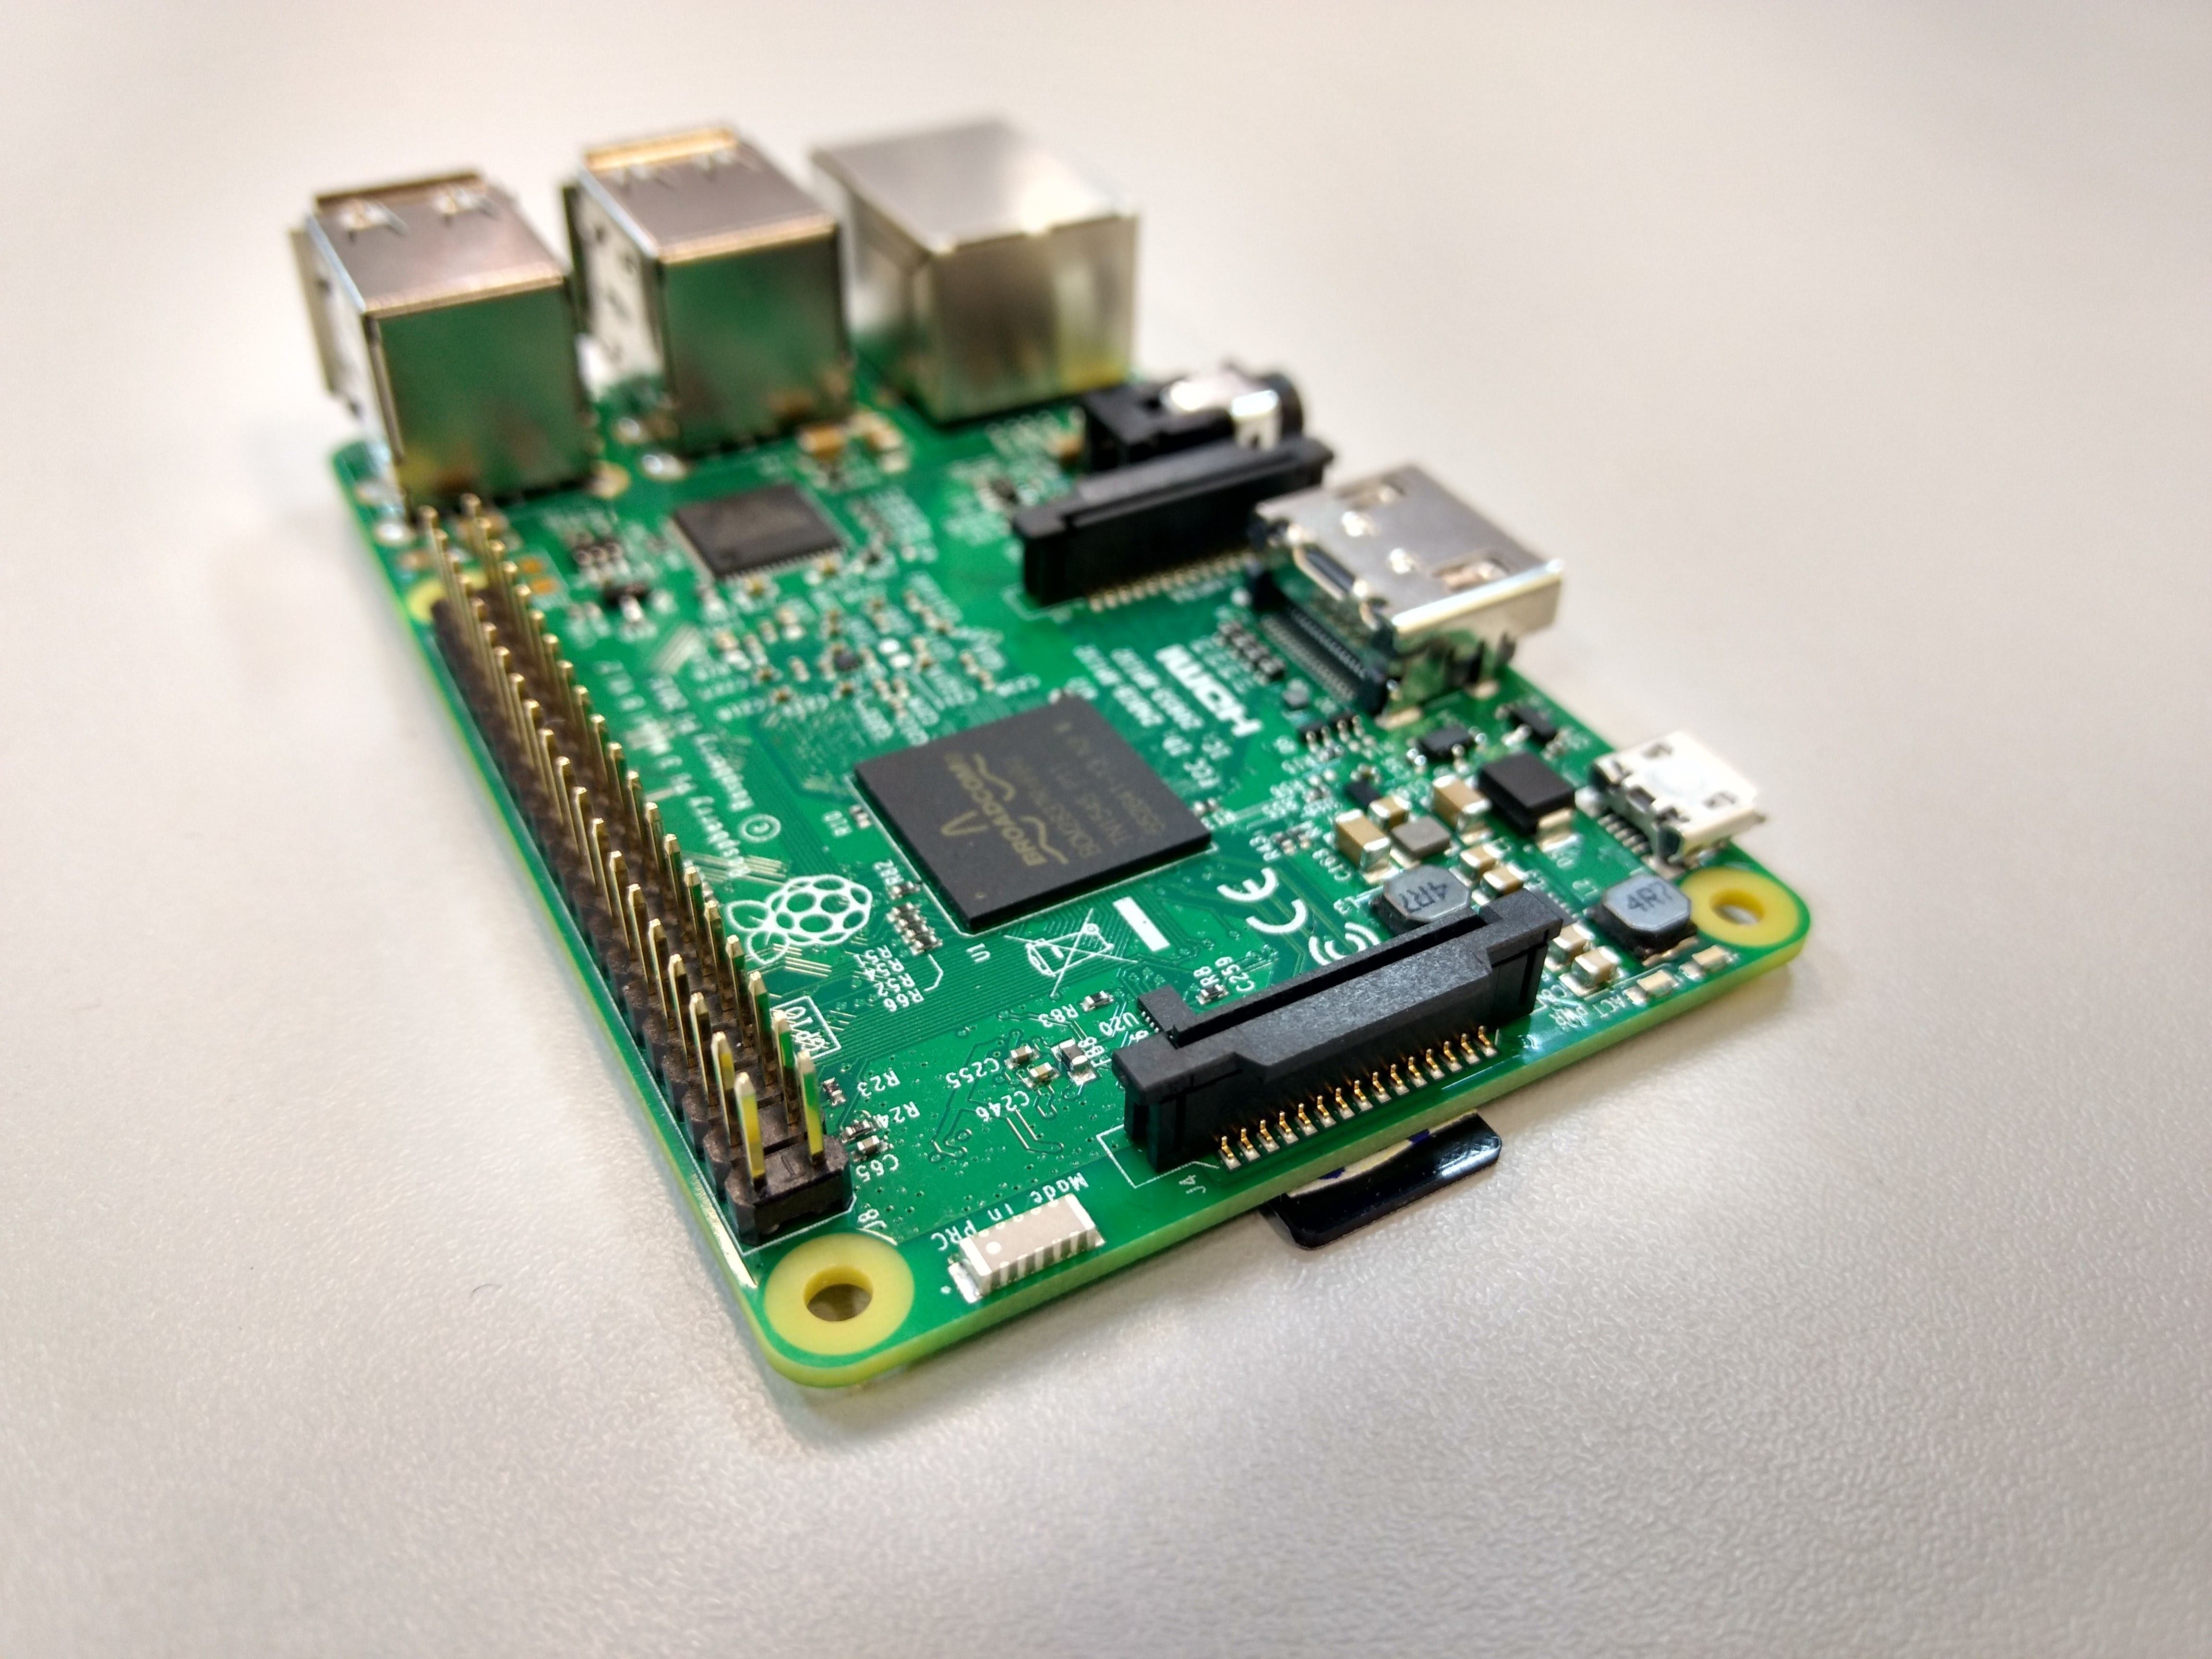
\includegraphics[width=1\textwidth]{040-plataformas/RPi-Wi-Fi-dongles/rpi-onboard.jpg}
	\end{center}
	\legend{Fonte: Elaborada pelo autor}
\end{figure}

Após o desenvolvimento e testes com ESP8266, foi testado e desenvolvido
software para transformar o Raspberry Pi em uma plataforma para hospedar o
sensor. Sua principal diferença é o sistema operacional linux (inexistente no
ESP8266) que favorece o Raspberry e o alto custo que o desfavorece. Em média no
exterior o Raspberry Pi é vendido por USD \$ 35,00 \cite{RPI2016}
e no Brasil entre R\$ 270 em Março de 2016 e R\$ 190 em Janeiro de 2017 \cite{rpi3-mercadolivre}.

As vantagens de ter um computador moderno completo sobrepõem seu custo em muitas
vezes. Dentre as quais destacamos a interface "amigável" com usuário devido ao
sistema operacional oferecendo maior nível de abstração (bastando apenas alguns
comandos para acessá-los realizar tarefas complexas), comunidade \emph{open
source} e o poder computacional.
Além deste recurso a nível de sistema, a comunidade e número de projetos "faça
você mesmo" é muito maior que a do ESP8266, devido a sua simplicidade em
conectar-se a um monitor e construir protótipos e aplicações.


\subsection{Disponibilidade no mercado}
\label{subsec:mercado-esp}



O Raspberry é ligado por uma fonte de 2A, 5V e 10W através de uma entrada micro
USB. Para ligá-la, foi adquirido uma fonte USB tipo A para iPad, pois além de
poder desconectar o cabo da fonte, facilitando a manutenção, fornece a
quantidade exata de amperagem que o computador precisa. A primeira aquisição foi
de um carregador de \emph{smartphone} que não forneceu os amperes necessários.

Figura x.x - Carregador USB
![](carregador-ipad.jpg)


**Sistema Operacional**

O Raspberry Pi comporta diversos sistemas operacionais que são carregados de seu
cartão \emph{microSD}. Alguns exemplos de sistemas compatíveis:
\emph{Archlinux}, \emph{OpenELECE}, \emph{Raspbian}, \emph{Risc OS},
\emph{Pidora}, \emph{Kali Linux}, \emph{Windows 10 IoT}, entre outros. Para este
trabalho, foi utilizado o \emph{Raspbian} cuja interface é mostrada na
\selfref{fig:raspbian-jessie}.

\begin{figure}[htb]
	\caption{\label{fig:raspbian-jessie}Raspbian Jessie com Pixel}
	\begin{center}
		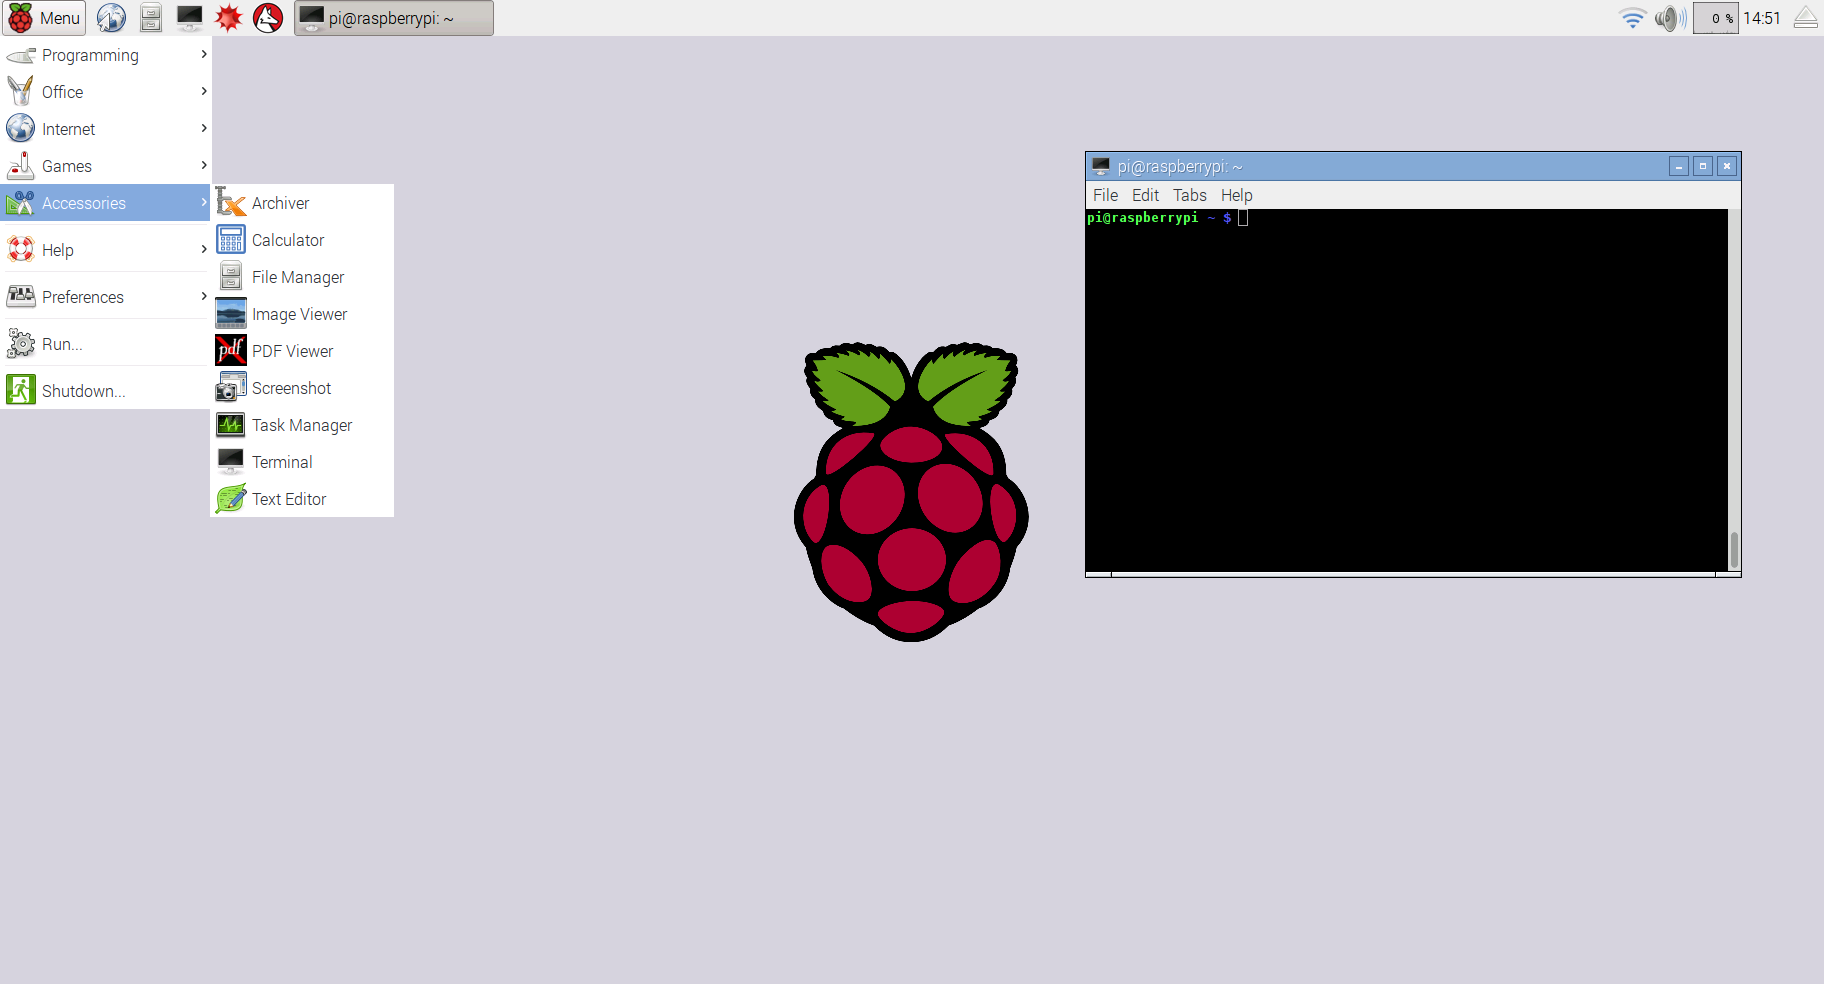
\includegraphics[width=1\textwidth]{040-plataformas/RPi-Wi-Fi-dongles/raspbian.jpg}
	\end{center}
	\legend{Fonte: Elaborada pelo autor}
\end{figure}



\subsection{Desenvolvimento e Implantação}
\label{subsec:dev-esp}


\subsection{Testes e resultados}
\label{subsec:mercado-esp}



**Conclusão sobre Raspberry Pi**

O Raspberry foi adotado como o sensor para detectar os dispositivos. O modo
promíscuo conseguiu ser acessado através de adaptador/módulo USB Wi-Fi. Mais
detalhes sobre a construção e adoção deste computador serão apresentados no
capítulo "Construção".

**Comparativo RPi X ESP8266**

Em comparação com o ESP8266, o Raspberry Pi compensou seu preço mais caro devido
a facilidade de programação e acesso aos seus recursos e integração e acesso a
recursos externos. Além disso, foi possível chegar ao modo promíscuo facilmente
através do Bash e do sistema operacional. A seguir, uma tabela comparando as
principais características do RPi e do módulo ESP12F.

Figura X.X - RPi x ESP12F
![](rpi-esp.png)
Fonte: Elaborada pelo autor.
